%% example on how to properly add a picture
% \begin{figure}[h]
%     \centering
%     \includegraphics[width=\linewidth]{example.png}
%     \caption{example}
%     \label{fig:example}
% \end{figure}

% %  example on how to properly add a code snippet
% \begin{lstlisting}[language=Python]
%     <insert code here>
% \end{lstlisting}
    
    

The core idea behind this thesis is to apply forecasting methods on the data from the real LoRaWAN deployment in Svebølle, Denmark.
Throughout this chapter, topology of the network as well as the communication model of the network will be explained.
Also, data processing, cleaning and transforming methods prior to the modeling are explained. 
The idea of modeling the transformed data is to examine whether there is a possibility of predicting future activation of event-driven end devices.
The activation of the end device is characterized as a successful uplink data transmission and proposed model for predicting is LSTM, an artificial recurrent neural network architecture widely used in the field of deep learning on sequential data.

The reasons for the activity prediction are diverse but knowing the probability of activation for given future time interval can help a great deal in the battery life savings.
There are usually thousands of devices connected in the single IoT network and improving energy efficiency is important research topic to deal with. 
One example the improving of the battery life for this deployment could be strategic positioning of the end device regards to the base station. 
Placing the base station near the devices that are more likely to transmit data could lead to decrease of the package time-on-air (ToA).


\section{Network topology of the deployment in Svebølle, Denmark}
As previosly defined, the LoRaWAN topology is a star-of-stars type where each end device is connected and transmit data to the base station (or multiple stations) and the base station is connected via higher bandwidth protocol to the network server.
The network server decodes the packets received from the base station and after performing security checks transmits data to theapplication server.
The application server is usually hosted on cloud infrastructure platforms such as Google Cloud, Amazon Web Server or Azure.

This thesis uses data measurued on the base station end of the LoRaWAN network deployment in Svebølle, Denmark. 
End devices are set on city lights and there is a single base station, network deployment in fig. \ref{fig:svebolle}.
\begin{figure}[h]
    \centering
    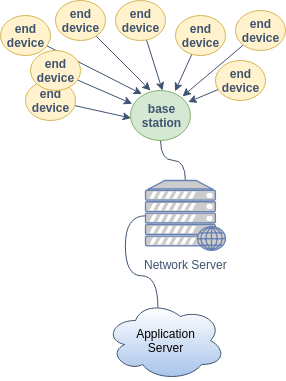
\includegraphics[width=0.5\linewidth]{Svebolle-Topology.png}
    \caption{Overview of the network topology of the LoRaWAN deployment on city lights in Svebølle}
    \label{fig:svebolle}
\end{figure}
Atmospheric data is collected and sent sporadically to the base station.
Base station collected the data with the encrypted MAC payload where relevant attributes are:
\begin{itemize}
    \item \textit{time} - in datetime format to microsecond precision
    \item \textit{DevAddr} - end device public 32-bit address wirten in HEX format
    \item \textit{freq} - radio frequency of the carrier signal
    \item \textit{chan} - used channel
    \item \textit{BW} - bandwidth
    \item \textit{SPF} - spreading factor
    \item \textit{RSSI} - received signal strength indication
    \item \textit{SNR} - signal-to-noise ratio
    \item \textit{CR} - code rate
    \item \textit{DR} - data rate
    \item \textit{CRCstatus} - flag that indicates if there were transmission error
    \item \textit{mType} - type of MAC message
    \item \textit{MACPayload} - the actual, intended message in encrypted form
\end{itemize}

The communication model is depicted in fig. \ref{fig:sv_cm}.
\begin{figure}[h]
    \centering
    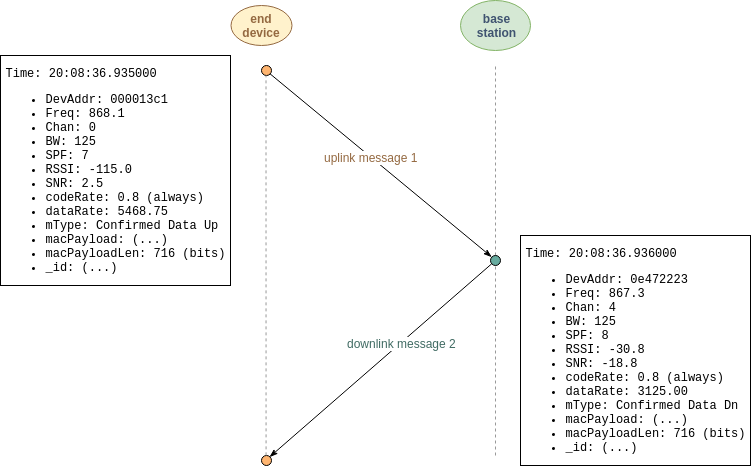
\includegraphics[width=\linewidth]{Svebolle-ed-bs-model.png}
    \caption{Two-way communication model between the end device and the base station in the LoRaWAN deployment in Svebølle. Due to the nature of communication, end devices can be classified as Class A devices which support bi-directional communication between a device and a base station}
    \label{fig:sv_cm}
\end{figure}
Uplink messages (messages sent by an end device to the base station) can be sent at any time and there is no regular pattern in uplink transmissions. 
Downlink messages happen when devices open receiving windows at specified times (1s and 2s) after an uplink transmission.
If there is no response from the server, the next opportunity will be after the next uplink transmission from an end device.

\section{Measured data}
The measurement took place during a five month period where about six hundred thousand data points were captured on the base station end.
The data set contains 250 unique device addresses where there is large disproportion between the number of transmission for each device. 
The data known prior to transmission is device address, frequency of the carrier signal, channel, bandwidth, spreading factor, code rate and message type as well as MAC payload.
On the receiver end (base station) RSSI and SNR are captured.
Statistical inference, the process of deducing properties of an underlying probability distribution, is shown in fig. \ref{fig:fit}. 
\begin{figure}[h]
    \centering
    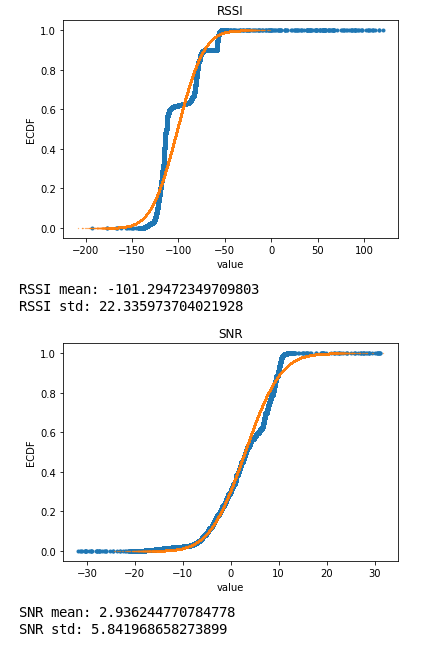
\includegraphics[width=0.6\linewidth]{fit.png}
    \caption{RSSI and SNR value distribution in comparisson to theoretical Rician distribution. Blue dotted plot represents the actual measured data, while orange line represents the Rician theoretical distribution}
    \label{fig:fit}
\end{figure}
We use statistical inference to make probabilistic conclusions about what can be expected if the data is collected again.
If the theoretical distribution is fitting the measured data, we will be able to draw acceptable conclusions from the data and give more general conclusions from relatively few data points.
In fig. \ref{fig:fit}, there is a comparisson between the actual distribution and the Rice theoretical distribution but due to the high irregularity in the measured data, it doesn't make a perfect fit.


\section{Data preprocessing and transformation to a time series format}
Due to the nature of the problem of the future activation prediction for each end device, many of the captured attributes are irrelevant.
The measurements in the data set are not structured as a time series data, only moments when transmission of LoRa messages were successful in uplink direction were captured and stored.
Since time series data is a series of data points indexed in time order and taken at successive equally spaced points in time, the data set had to be processed.
The only important label in the processed data set is the flag which indicates wheter the end device sucessfully transmitted the message to the base station or not.
For each time point, where every time point is observation in seconds, there is an activity flag assigned.
If the device was active for observed time point, the activity flag is 1, otherwise the activity flag is 0.
Since the measurements were carried out through long period, newly created data set was large enough to be suitable candidate for applying deep learning methods to perform forecasting of future time points.

Above described process was carried out using Python 3.7.1 programming language using following methods:
\begin{itemize}
    \item extracting the only important features from the data set, \textit{Time} of the event and \textit{DevAddr}, which stands for 32-bit public end device address. The data set was preloaded into the data frame, two-dimensional size-mutable, potentially heterogenous tabular data structure with labeled axes \cite{df} .
    \begin{lstlisting}[language=Python]
        def get_features(df):
            return df[['Time', 'DevAddr']]
    \end{lstlisting}
    \item lowering time resolution from nanosecond precision to second precision, which means if input is 2017-01-02 12:08:27.788000, output will be 2017-01-02 12:08:27.
    \begin{lstlisting}[language=Python]
        def clean_features(df):
            Time = list(df.Time.values)
            Time_parsed = []
            sep = '.'
            for t in Time:
                t_parsed = t.split(sep, 1)[0]
                Time_parsed.append(t_parsed)
            df.Time = Time_parsed
            df['Time'] = pd.to_datetime(df['Time'])
            return df
    \end{lstlisting}
    \item selecting the device whose activity will be predicted
    \begin{lstlisting}[language=Python]
        def select_dev(df, dev_name='000013c1'):
            df = df[df.DevAddr == dev_name]
            df = df.reset_index(drop=True)
            df = df.Time
            df = df.drop_duplicates(keep='last')
            df = pd.DataFrame({'Time':df.values})
            return df
    \end{lstlisting}
    \item adding activaty flag 1
    \begin{lstlisting}[language=Python]
        def add_label(df):
            df['Active'] = 1
            return df
    \end{lstlisting}
    \item resampling data in order to achieve the time series format. For each second there is either flag 0 or 1 which indicates the device activity.
    \begin{lstlisting}[language=Python]
        def datetime_resampling(df):
            df = df.set_index('Time')
            df.index = pd.to_datetime(df.index)
            df = df.resample('1S').asfreq()
            df = df.fillna(0)
            return df
    \end{lstlisting}
\end{itemize}

Post-processed data set was stored in the data frame data structure with only two columns, one for the datetime and the other for the end device activation indicator.

\section{Proposed LSTM model for predicting future activation of end devices}
The LSTM model was developed using Keras, a high-level neural networks API, capable of running on top of Tensorflow.
Tensorflow is an open source software library for numerical computation using data flow graphs.
The graph nodes represent mathematical operations, while the graph edges represent the multidimensional data arrays (tensors) that flow between them \cite{tensorflow}.

The workflow of the neural network development is particulary well suited and fine-tuned for large-scale machine learning.
Its basic principle is very simple: first a graph of computations in Python has to be defined and then Tensorflow takes that graph and runs it efficiently using optimized C++ code \cite{Aurelian}.

Tensorflow allows the user to break up the graph into several chunks and run them in parrallel across many CPUs and GPUs.
Also, it supports distributed computing for creating and training large neural networks on the big data.

The created graph is shown in fig. \ref{fig:graph} and is described in detail in \autoref{chap:appendix}.
\begin{figure}[H]
    \centering
    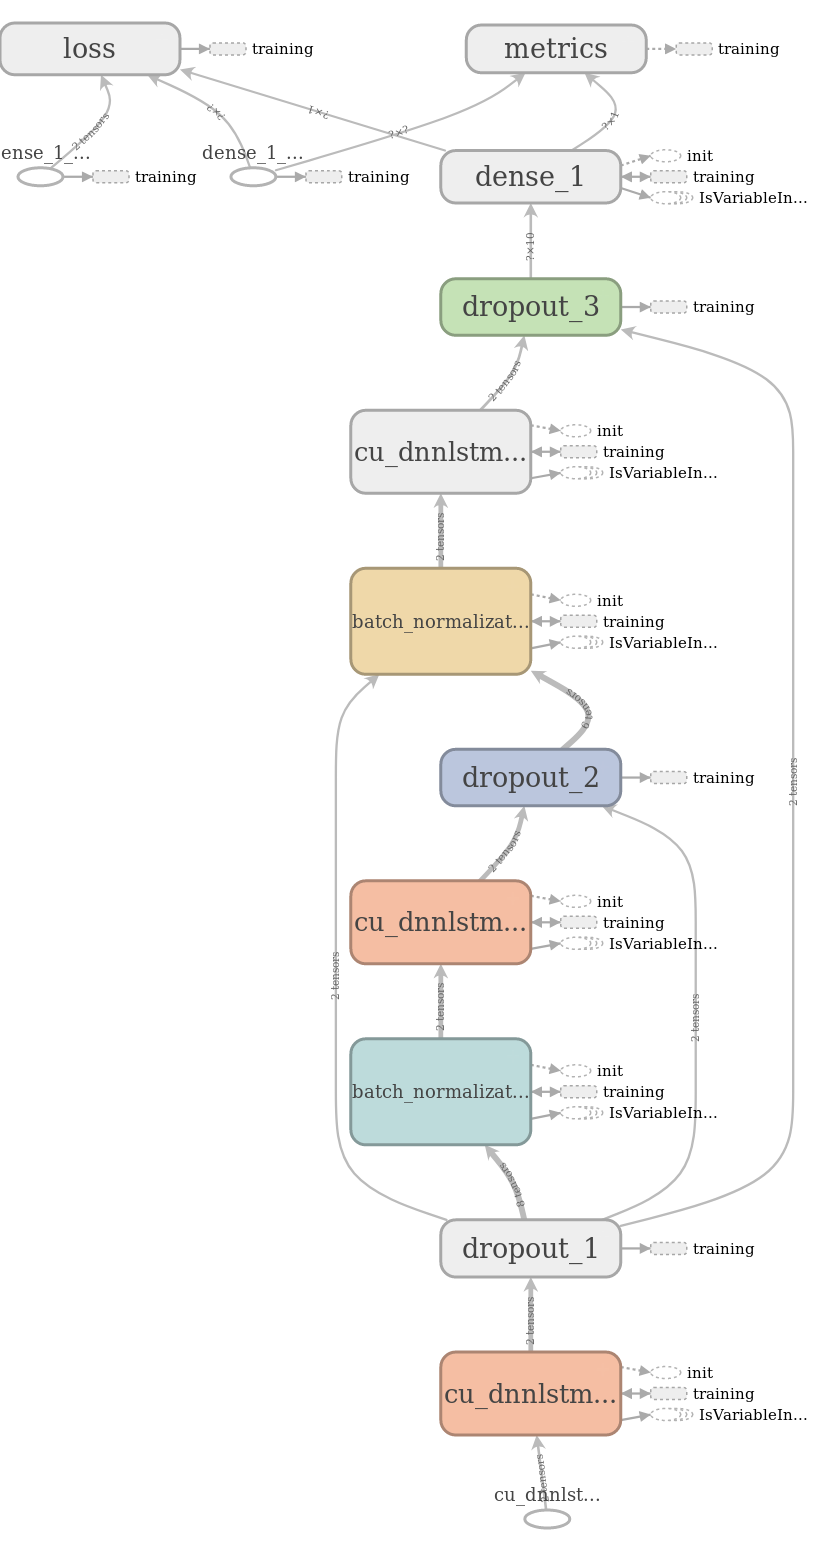
\includegraphics[width=0.7\linewidth]{graph.png}
    \caption{The dataflow graph representing the LSTM model created to predict the future end device activation using the large dataset described through the last chapter.
    The dataflow graph is used to represent the computation in terms of the dependencies between individual operations}
    \label{fig:graph}
\end{figure}
The Adam (Adaptive Moment Estimation) optimizer is used.
The Adam optimization algorithm is an extension to the stohastic gradient descent and it combines the best properties of AdaGrad and RMSProp algorithms to provide an optimization that can handle sparse gradients on noisy problems.

In order to implement the LSTM neural network, it is important to create the sequential network model.
The sequential model allows simultaneously taking a sequence of inputs and produce a sequence of outputs.
The data set is further processed to be able to fed the network.
From the processed time series data, time-delayed time series data is created using specific \textit{window size}.
If the window size is $n$, for every time point sequence of $n$ historical values will be created.
That means the activation of the current time point $y(t)$ is conditioned by the activation in moments $y(t-1), y(t-2), ..., y(t-n)$.
The following function shows how the time-delayed data set is created. $X$ is an array of sequences that each has $delay$ historical elements, while the $y$ is the array of elements that succeeds each of the respective sequnces from the $X$ array.
\begin{lstlisting}[language=Python]
    def timeDelay(df, delay):
        X_data, y_data = [], []
        
        for i in range(delay, len(df)):
            X_data.append(df[i-delay: i].tolist())
        X_data = np.array(X_data)
        y_data = df[delay:]
        return np.reshape(X_data, (X_data.shape[0],\
                                   X_data.shape[1], 1)),\
               np.reshape(y_data, (len(y_data), ))
\end{lstlisting}
This sequential model contains multiple layers of memory cells, thus creating a deep LSTM network.
After each LSTM layer, the dropout layer is applied. 

Dropout layers are added in order to prevent overfitting the training set, common issue for deep sequential neural networks.
Dropout was proposed in \cite{dropout} in 2012 and it has proven to be highly successful.
The dropout algorithm is a fairly simple one: at every training step, every neuron (including the input neurons but excluding the output neurons) has a probability $p$ of being temporarily \textit{dropped out}, meaning it will be entirely ignored during this training step, but it may be active during the next step. 
The hyperparameter $p$ is called the \textit{dropout rate}. 
After training session, neurons don't get dropped anymore \cite{Aurelian}.

The LSTM layer was realized as CuDNNLSTM, which is a fast LSTM implementation backed by cuDNN and can only be run on GPU.
The NVIDIA CUDA Deep Neural Network library (cdDNN) is a GPU-accelerated library of primitives for DNNs. cuDNN provides highly tuned implementations for standard routines such as back propagation, pooling, normalization and activation layers.
The first LSTM layer contains 128 neurons with added return sequnce, which returns the last output.
After the LSTM layer and the dropout layer comes batch normalization. 
Batch normalization normalizes the output of a previous activation layer by subtracting the batch mean and dividing by the batch standard deviation where batch is hardcoded to the value of 64.
The batch size defines the number of samples that will be propagated through the network.
The second layer is again represented as follows: the LSTM layer, dropout, batch normalization.
The last layer contains a small size LSTM layer with 10 neurons and without return sequence. 
Then again, droput is applied. 
Finally, the last part of the last layer is the dense single-neuron layer which performs multiplying the input value and the weight, adds a bias and activates the result.
The output is, in this case, a value between 0 and 1 for each input sequnce. 

The training process starts with all weights initialized randomly. 
During the training, random weights are changing due to some neural network performance metrics. 
Usually, this performance metrics is observed in terms of loss function. 
Loss function is a function that defines accuracy for trained network and should be much lower in the end of the training.
Thus, the problem of training is equivalent to the problem of minimizing the loss function. 
This model has the MSE (mean square error) function implemented and training was done through 10 epochs where each epoch is one forward pass and one backward pass of all training examples.

\section{Results}
\subsection{Output interpretation}
The described LSTM model is usually used for the time series where each time point on x-axis has some value attached to the y-axis. 
In terms of machine learning, this model is best for the regression problem where the concrete value of the future moment will be predicted.
Mainly, an LSTM network is used in the natural language processing (NLP), weather forecasting, stock predictions or any basic regression task applied to the time series data. 
For this data set, the problem is more of a classification nature than it is a regression task. 
We want to create the predictions of the activation for each end device in the LoRaWAN deployment where the activation is a \textit{bool} value that indicates if the transmission is going to happen (1) or not (0).

After the training process, the validation on the test set was done.
The data set of sequnces created using \textit{timeDelayed} function was split on the train and the set in the 80:20 ratio using the following function:
\begin{lstlisting}[language=Python]
    def split(X, y, ratio):    
        test_split = int(len(X) * ratio)
        
        X_train, y_train = X[:test_split], y[:test_split]
        X_test, y_test = X[test_split:], y[test_split:]
        return X_train, y_train, X_test, y_test
\end{lstlisting}
Since the last layer is a single-neuron dense layer with linear activation function, the output was not defined as binary output (classification) but rather as any value from 0 to 1.
For the described model trained in 10 epochs with the time delay of 5 historical values, the output was the following array (considering only a single device, with no multivariate analysis):
\begin{lstlisting}[language=Python]
    array([[1.21673493e-05, 5.82448400e+06],
           [1.52176805e-03, 2.00000000e+01],
           [1.84416212e-03, 2.00000000e+01],
           [1.91396230e-03, 2.00000000e+01],
           [1.91468524e-03, 2.00000000e+01],
           [1.91875699e-03, 2.00000000e+01]])
\end{lstlisting}
There is an obvious difference between those values and the interpretation was done using the following code:
\begin{lstlisting}[language=Python]
    y_test_pred_10[y_test_pred_10==1.21673493e-05]=0
    y_test_pred_10[y_test_pred_10!=0]=1
\end{lstlisting}
In fig. \ref{fig:output}, the predicted data after the interpretation and the actual data of the test set are depicted.
\begin{figure}[h]
    \centering
    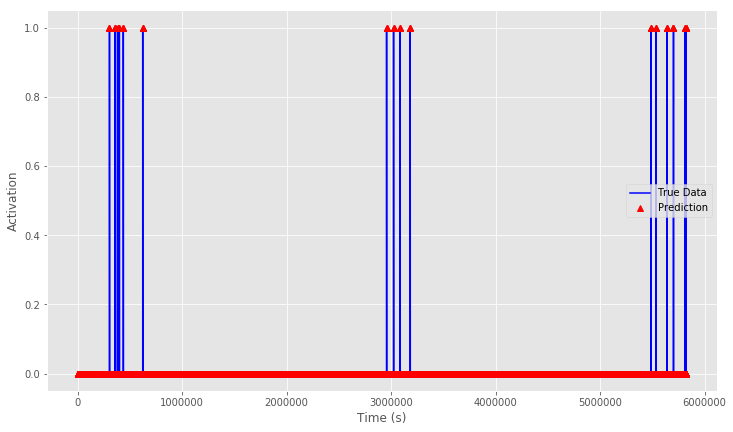
\includegraphics[width=\linewidth]{output.png}
    \caption{The processed LSTM output is represented with red triangles, which estimate moments in which observed device is active (1) or not active (0), while blue lines represent the actual device activation}
    \label{fig:output}
\end{figure}

Since this problem cannot be considered classification nor regression, it is hard to define the error metric.
The idea was to determine how far the predicted data is from the actual value in seconds.
In most cases it is 1 to 5 seconds but the worst case scenario is depicted in fig. \ref{fig:err}.
\begin{figure}[h]
    \centering
    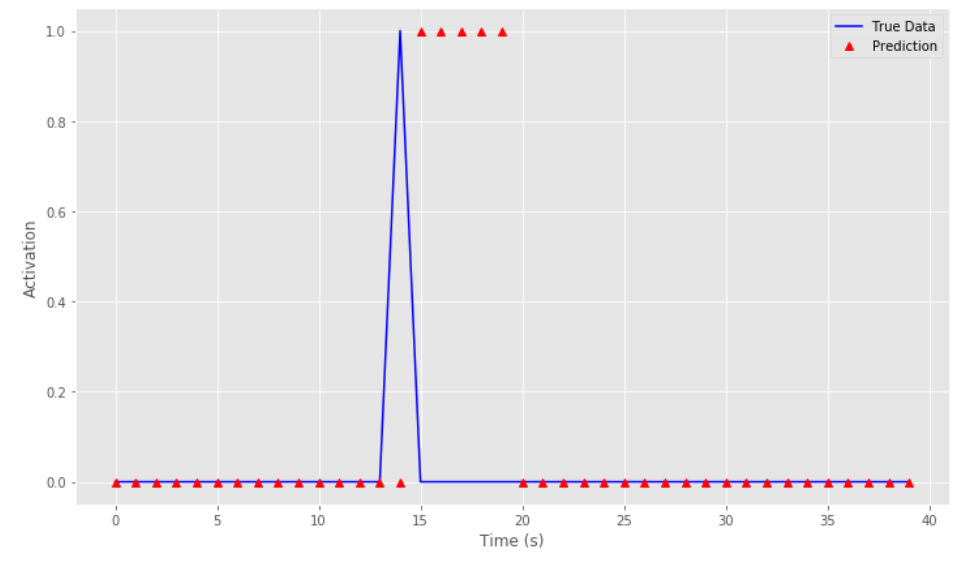
\includegraphics[width=\linewidth]{err.png}
    \caption{Error predictions for some time points not only miss the moment of the actual activation but also they are multiplied by the number of the delay initialized in the process of creating the time-delayed time series data set for training}
    \label{fig:err}
\end{figure}
For some events network predicts activation very close to the actual activation but multiplies number of events by the number of delay performed in the creation of time-delayed data set, in this case by 5.

The root mean square error (RMSE) between moments of the actual activation versus the predicted activation is a bit below 2s.
To put the RMSE rate in context, the RMSE value is compared to time difference between two activations.
In fig. \ref{fig:err_con}, the histogram of time differences is shown.
The vertical line represents the RMSE value.
If the occasional multiplication of predicted activations is ignored, the histogram could be a good error indicator.
The left area of the histogram is the percentage of mispredicted activations, while the right area of the histogram is the percentage of correctly predicted end device activations. 
The percentage of mispredicted activations (the error percentage) is 0.35\%.

\begin{figure}[H]
    \centering
    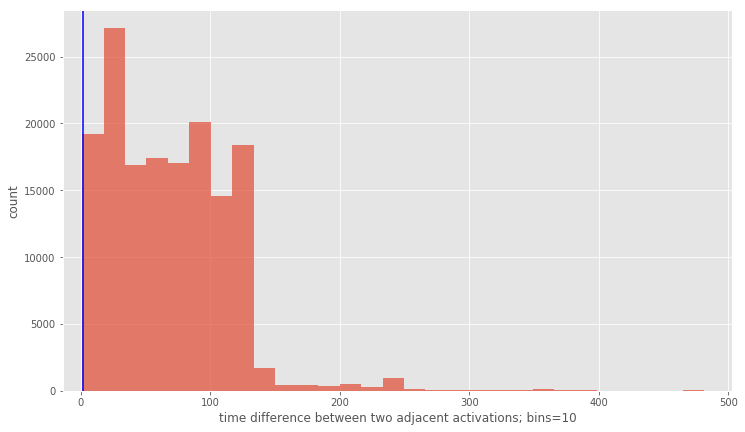
\includegraphics[width=\linewidth]{err_con.png}
    \caption{Histogram of time differences for each two adjacent end device activations}
    \label{fig:err_con}
\end{figure}

\subsection{Probability estimation of activation of the end device in a future arbitrarily-large time interval}
The core idea of the thesis is not to be able to create accurate predictions for a single point, but rather to create the probability estimation of the end device activation in a future time interval.
The general hypothesis is defined as follows: for the given period of time ($n$ seconds), the probability of the end device activation (transmission of the LoRa uplink message) should rise up as a time period gets bigger.
$$ n = 0 \Rightarrow p_{a} = 0 $$
$$ n \in <0, +\infty> \Rightarrow p_{a} \in <0, 1> $$
$$ n = \infty \Rightarrow p_{a} = 1 $$
where $n$ is the number of seconds of the future time interval for which the probability of an end device activation, $p_{a}$, will be calculated.

The algorithm for calculating the probability of the end device activation based on predicted data set is defined in the following code:
\begin{lstlisting}[language=Python]
    def estimate_prob(data, window_size):
        windows = gen_window(data, n=window_size)

        window_prob = []

        for window in windows:
            ones_freq = 0
            for data_point in window:
                if data_point == 1:
                    ones_freq += 1
            window_prob.append(ones_freq/window_size)
        return 1 - window_prob.count(0.0)/len(window_prob)
\end{lstlisting}
where the function takes two parameters, the predicted and processed output of the LSTM model as \textit{data} and the arbitrarily sized time window (number of seconds) as \textit{window\_size} for which the estimation of the probability of the end device activation will be calculated.
Considering the size of the window, \textit{windows} list is generated using the function \textit{gen\_window} which yields a sliding window over data from the iterable sequnce of data. 
The \textit{gen\_window} function:
\begin{lstlisting}[language=Python]
    def gen_window(seq, n):
        it = iter(seq)
        result = tuple(islice(it, n))
        if len(result) == n:
            yield result
        for elem in it:
            result = result[1:] + (elem,)
            yield result
\end{lstlisting}
For each \textit{window} in the list of \textit{windows} the number of activation is counted and the probability of the activation is calculated.
The final prediction is calculated as the mean of activation probabilites for each time window.
In fig. \ref{fig:prob}, it is shown how the probability of the end device activation based on the predicted data set is increasing with time.
\begin{figure}[h]
    \centering
    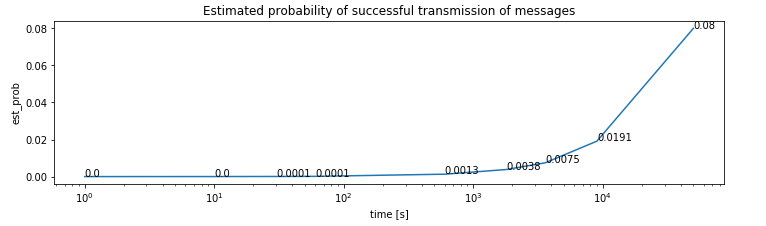
\includegraphics[width=\linewidth]{est-prob.png}
    \caption{The estimation of the probability of a single end device activation on the test data}
    \label{fig:prob}
\end{figure}